% Options for packages loaded elsewhere
\PassOptionsToPackage{unicode}{hyperref}
\PassOptionsToPackage{hyphens}{url}
\PassOptionsToPackage{dvipsnames,svgnames,x11names}{xcolor}
%
\documentclass[
  letterpaper,
  DIV=11,
  numbers=noendperiod]{scrartcl}

\usepackage{amsmath,amssymb}
\usepackage{iftex}
\ifPDFTeX
  \usepackage[T1]{fontenc}
  \usepackage[utf8]{inputenc}
  \usepackage{textcomp} % provide euro and other symbols
\else % if luatex or xetex
  \usepackage{unicode-math}
  \defaultfontfeatures{Scale=MatchLowercase}
  \defaultfontfeatures[\rmfamily]{Ligatures=TeX,Scale=1}
\fi
\usepackage{lmodern}
\ifPDFTeX\else  
    % xetex/luatex font selection
\fi
% Use upquote if available, for straight quotes in verbatim environments
\IfFileExists{upquote.sty}{\usepackage{upquote}}{}
\IfFileExists{microtype.sty}{% use microtype if available
  \usepackage[]{microtype}
  \UseMicrotypeSet[protrusion]{basicmath} % disable protrusion for tt fonts
}{}
\makeatletter
\@ifundefined{KOMAClassName}{% if non-KOMA class
  \IfFileExists{parskip.sty}{%
    \usepackage{parskip}
  }{% else
    \setlength{\parindent}{0pt}
    \setlength{\parskip}{6pt plus 2pt minus 1pt}}
}{% if KOMA class
  \KOMAoptions{parskip=half}}
\makeatother
\usepackage{xcolor}
\setlength{\emergencystretch}{3em} % prevent overfull lines
\setcounter{secnumdepth}{5}
% Make \paragraph and \subparagraph free-standing
\makeatletter
\ifx\paragraph\undefined\else
  \let\oldparagraph\paragraph
  \renewcommand{\paragraph}{
    \@ifstar
      \xxxParagraphStar
      \xxxParagraphNoStar
  }
  \newcommand{\xxxParagraphStar}[1]{\oldparagraph*{#1}\mbox{}}
  \newcommand{\xxxParagraphNoStar}[1]{\oldparagraph{#1}\mbox{}}
\fi
\ifx\subparagraph\undefined\else
  \let\oldsubparagraph\subparagraph
  \renewcommand{\subparagraph}{
    \@ifstar
      \xxxSubParagraphStar
      \xxxSubParagraphNoStar
  }
  \newcommand{\xxxSubParagraphStar}[1]{\oldsubparagraph*{#1}\mbox{}}
  \newcommand{\xxxSubParagraphNoStar}[1]{\oldsubparagraph{#1}\mbox{}}
\fi
\makeatother


\providecommand{\tightlist}{%
  \setlength{\itemsep}{0pt}\setlength{\parskip}{0pt}}\usepackage{longtable,booktabs,array}
\usepackage{calc} % for calculating minipage widths
% Correct order of tables after \paragraph or \subparagraph
\usepackage{etoolbox}
\makeatletter
\patchcmd\longtable{\par}{\if@noskipsec\mbox{}\fi\par}{}{}
\makeatother
% Allow footnotes in longtable head/foot
\IfFileExists{footnotehyper.sty}{\usepackage{footnotehyper}}{\usepackage{footnote}}
\makesavenoteenv{longtable}
\usepackage{graphicx}
\makeatletter
\def\maxwidth{\ifdim\Gin@nat@width>\linewidth\linewidth\else\Gin@nat@width\fi}
\def\maxheight{\ifdim\Gin@nat@height>\textheight\textheight\else\Gin@nat@height\fi}
\makeatother
% Scale images if necessary, so that they will not overflow the page
% margins by default, and it is still possible to overwrite the defaults
% using explicit options in \includegraphics[width, height, ...]{}
\setkeys{Gin}{width=\maxwidth,height=\maxheight,keepaspectratio}
% Set default figure placement to htbp
\makeatletter
\def\fps@figure{htbp}
\makeatother
% definitions for citeproc citations
\NewDocumentCommand\citeproctext{}{}
\NewDocumentCommand\citeproc{mm}{%
  \begingroup\def\citeproctext{#2}\cite{#1}\endgroup}
\makeatletter
 % allow citations to break across lines
 \let\@cite@ofmt\@firstofone
 % avoid brackets around text for \cite:
 \def\@biblabel#1{}
 \def\@cite#1#2{{#1\if@tempswa , #2\fi}}
\makeatother
\newlength{\cslhangindent}
\setlength{\cslhangindent}{1.5em}
\newlength{\csllabelwidth}
\setlength{\csllabelwidth}{3em}
\newenvironment{CSLReferences}[2] % #1 hanging-indent, #2 entry-spacing
 {\begin{list}{}{%
  \setlength{\itemindent}{0pt}
  \setlength{\leftmargin}{0pt}
  \setlength{\parsep}{0pt}
  % turn on hanging indent if param 1 is 1
  \ifodd #1
   \setlength{\leftmargin}{\cslhangindent}
   \setlength{\itemindent}{-1\cslhangindent}
  \fi
  % set entry spacing
  \setlength{\itemsep}{#2\baselineskip}}}
 {\end{list}}
\usepackage{calc}
\newcommand{\CSLBlock}[1]{\hfill\break\parbox[t]{\linewidth}{\strut\ignorespaces#1\strut}}
\newcommand{\CSLLeftMargin}[1]{\parbox[t]{\csllabelwidth}{\strut#1\strut}}
\newcommand{\CSLRightInline}[1]{\parbox[t]{\linewidth - \csllabelwidth}{\strut#1\strut}}
\newcommand{\CSLIndent}[1]{\hspace{\cslhangindent}#1}

\KOMAoption{captions}{tableheading}
\makeatletter
\@ifpackageloaded{caption}{}{\usepackage{caption}}
\AtBeginDocument{%
\ifdefined\contentsname
  \renewcommand*\contentsname{Table of contents}
\else
  \newcommand\contentsname{Table of contents}
\fi
\ifdefined\listfigurename
  \renewcommand*\listfigurename{List of Figures}
\else
  \newcommand\listfigurename{List of Figures}
\fi
\ifdefined\listtablename
  \renewcommand*\listtablename{List of Tables}
\else
  \newcommand\listtablename{List of Tables}
\fi
\ifdefined\figurename
  \renewcommand*\figurename{Figure}
\else
  \newcommand\figurename{Figure}
\fi
\ifdefined\tablename
  \renewcommand*\tablename{Table}
\else
  \newcommand\tablename{Table}
\fi
}
\@ifpackageloaded{float}{}{\usepackage{float}}
\floatstyle{ruled}
\@ifundefined{c@chapter}{\newfloat{codelisting}{h}{lop}}{\newfloat{codelisting}{h}{lop}[chapter]}
\floatname{codelisting}{Listing}
\newcommand*\listoflistings{\listof{codelisting}{List of Listings}}
\makeatother
\makeatletter
\makeatother
\makeatletter
\@ifpackageloaded{caption}{}{\usepackage{caption}}
\@ifpackageloaded{subcaption}{}{\usepackage{subcaption}}
\makeatother

\ifLuaTeX
  \usepackage{selnolig}  % disable illegal ligatures
\fi
\usepackage{bookmark}

\IfFileExists{xurl.sty}{\usepackage{xurl}}{} % add URL line breaks if available
\urlstyle{same} % disable monospaced font for URLs
\hypersetup{
  pdftitle={Frequent Inspections Fail to Curb Violations in Toronto's Good-Standing Food Establishments},
  pdfauthor={Jerry Xia},
  colorlinks=true,
  linkcolor={blue},
  filecolor={Maroon},
  citecolor={Blue},
  urlcolor={Blue},
  pdfcreator={LaTeX via pandoc}}


\title{Frequent Inspections Fail to Curb Violations in Toronto's
Good-Standing Food Establishments\thanks{Code and data are available at:
\url{https://github.com/Jerryx2020/toronto_dinesafe_analysis}}}
\author{Jerry Xia}
\date{September 27, 2024}

\begin{document}
\maketitle
\begin{abstract}
This study analyzes inspection patterns and compliance outcomes using
Toronto's DineSafe dataset (2022-2024) to explore the relationship
between inspection frequency and food safety infractions in restaurants
and takeout establishments. The data reveals that restaurants have a
higher percentage of inspections resulting in infractions compared to
takeout establishments, highlighting more significant compliance
challenges in full-service operations. These findings suggest that
current regulatory practices may need to focus more on restaurants to
ensure public safety. By identifying gaps in inspection frequency and
infractions, this analysis highlights the need for more targeted
oversight to improve food safety.
\end{abstract}

\renewcommand*\contentsname{Table of contents}
{
\hypersetup{linkcolor=}
\setcounter{tocdepth}{3}
\tableofcontents
}

\section{Introduction}\label{introduction}

In large urban centers like Toronto, ensuring food safety is a critical
public health priority. Foodborne illnesses pose significant risks, and
the health of the population is closely tied to the hygienic practices
of food establishments, including restaurants, food trucks, and takeout
locations. To address this, the DineSafe program, managed by Toronto
Public Health, enforces health and safety regulations by conducting
regular inspections of all food service establishments (Gelfand 2022).
These inspections result in outcomes ranging from a pass to a
conditional pass or even closure, depending on the establishment's
compliance with food safety standards. According to the Centers for
Disease Control and Prevention (CDC), frequent and transparent food
inspections are instrumental in reducing foodborne illness outbreaks, as
public posting of inspection results can encourage better compliance in
food service settings (Centers for Disease Control and Prevention 2024).
Despite this, significant variations exist in the frequency of
inspections and the severity of infractions, raising concerns about
whether some establishments, particularly mobile or temporary food
vendors, receive adequate regulatory attention (Analytics 2023).

This study focuses on analyzing Toronto's DineSafe dataset, covering
inspections from 2022 to 2024, to investigate patterns in inspection
frequency and compliance outcomes among different types of food
establishments. While previous research has broadly examined compliance
across food establishments, this paper delves deeper into the
relationships between establishment types---such as traditional
restaurants and takeout locations---and the severity of infractions
identified during inspections. Restaurants exhibit a higher rate of
severe infractions compared to takeout establishments, suggesting that
full-service operations may require more regulatory oversight to address
food safety challenges (Agency 2023).

To address this gap, the DineSafe inspection data for Toronto food
establishments was obtained and cleaned as described in
Section~\ref{sec-data-overview}. The results, presented in
Section~\ref{sec-data-results}, reveal key trends in the frequency of
inspections and the prevalence of infractions across different
establishment types. The findings indicate that while mobile food
vendors undergo fewer inspections than restaurants, they exhibit a
higher rate of severe infractions relative to the number of inspections
conducted. These insights, as discussed in Section~\ref{sec-discussion},
highlight the need for more frequent inspections or stricter regulations
in this sector to ensure public safety.

The remainder of this paper is organized as follows:
Section~\ref{sec-data-overview} provides a detailed overview of the data
and the methodology used to clean and analyze the dataset;
Section~\ref{sec-data-results} presents the key findings of the
analysis, including the inspection frequency and infraction severity;
and Section~\ref{sec-discussion} concludes with recommendations for
improving food safety oversight in Toronto. The appendix includes
additional materials, such as code and data, ensuring full
reproducibility of the results.

\section{Data}\label{sec-data}

\subsection{Overview}\label{sec-data-overview}

This analysis utilizes the DineSafe dataset from Toronto's Open Data
platform, accessed using the \texttt{opendatatoronto} package (Gelfand
2022). The dataset includes inspections conducted from 2022 to 2024,
providing detailed information on health inspections of food
establishments, including restaurants and takeout locations, throughout
Toronto. Key variables in the dataset include inspection dates,
infraction types, and establishment compliance statuses, which serve as
the primary indicators for assessing food safety. These regular
inspections are crucial for maintaining food hygiene standards, as
highlighted by the CDC, which emphasizes the importance of routine
inspections and the public posting of results, such as letter grades, to
encourage compliance and reduce foodborne illnesses (Centers for Disease
Control and Prevention 2024).

For this study, only the inspection data for ``Restaurant'' and ``Food
Take Out'' establishments that passed their most recent inspection were
retained. This focus allows for an in-depth exploration of the
correlation between inspection frequency and the occurrence of
infractions in establishments that are deemed to be in compliance. The
DineSafe dataset is updated regularly by Toronto Public Health, and is
considered open data under Toronto's Open Data Licence
(Section~\ref{sec-appendix-attribution}), as long as proper attribution
is provided (Toronto 2024).

The data analysis and processing were carried out using the R
programming language (R Core Team 2023), employing a range of
specialized packages. The \texttt{tidyverse} package (Hadley Wickham et
al. 2019) was used extensively for filtering, cleaning, and summarizing
the data. Additionally, the \texttt{ggplot2} package (H. Wickham 2016)
was applied to visualize patterns in inspection frequency and the
severity of infractions. Date-related data were managed using the
\texttt{lubridate} package (Grolemund and Wickham 2011) to ensure
consistency in handling inspection dates.

This analysis exclusively focuses on data for restaurants and takeout
establishments, as these are among the most common food service types in
Toronto, and represent a significant portion of the inspections carried
out by public health authorities. As described in
Section~\ref{sec-data-results}, the dataset was thoroughly cleaned and
prepared for analysis, ensuring that all irrelevant fields were removed
and the remaining data was formatted for accurate analysis.

\newpage

\subsection{Results}\label{sec-data-results}

\begin{figure}

\centering{

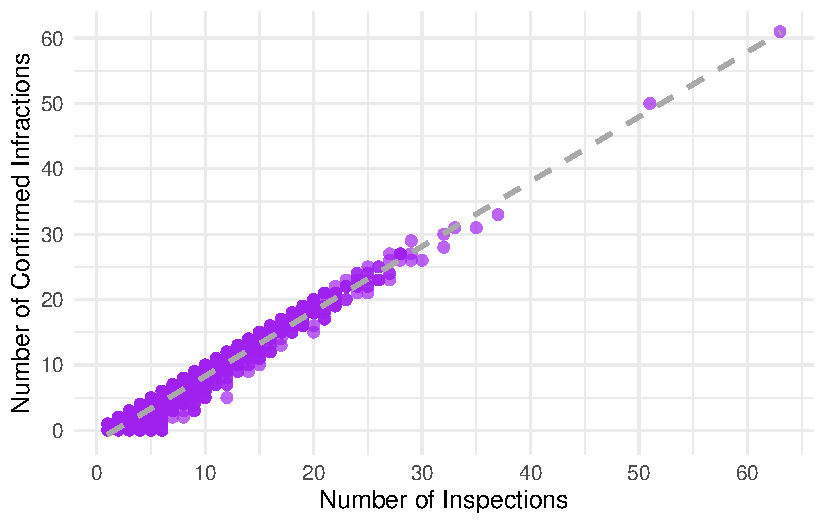
\includegraphics{paper_files/figure-pdf/fig-inspection-vs-infraction-1.pdf}

}

\caption{\label{fig-inspection-vs-infraction}Inspection Count vs
Infraction Count per Establishment}

\end{figure}%

As shown in Figure~\ref{fig-inspection-vs-infraction}, the graph now
excludes only inspections where ``No Infraction'' was recorded. The
results show that establishments inspected more frequently tend to have
higher counts of infractions. This positive correlation reflects
findings from the literature that increased inspection frequency does
not necessarily reduce violations but instead highlights pre-existing
issues (Public Health 2023; Centers for Disease Control and Prevention
2024). The data was processed using the \texttt{tidyverse} package for
summarization and visualization (Hadley Wickham et al. 2019), while the
plots were generated using \texttt{ggplot2} (H. Wickham 2016).

\newpage

\begin{figure}

\centering{

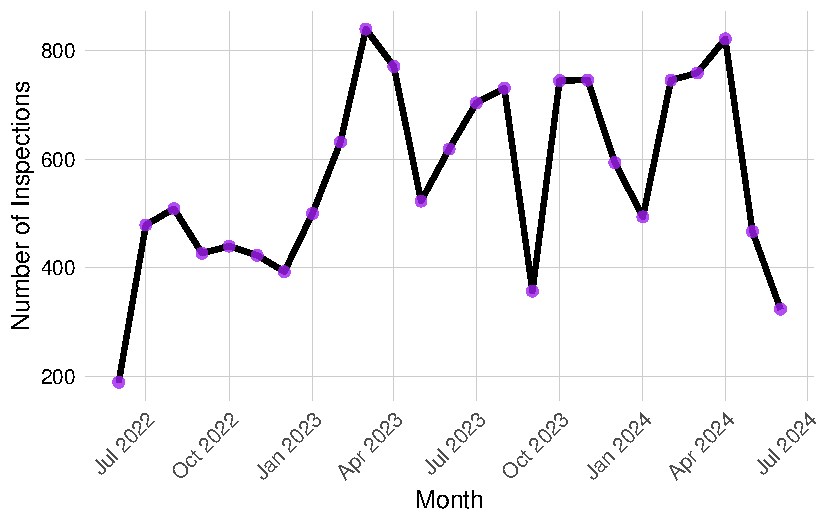
\includegraphics{paper_files/figure-pdf/fig-inspections-over-time-1.pdf}

}

\caption{\label{fig-inspections-over-time}Number of Inspections
Conducted Over Time (Monthly)}

\end{figure}%

As shown in Figure~\ref{fig-inspections-over-time}, the number of
inspections fluctuates month by month. Several external factors, such as
regulatory changes, seasonal variations, or public health crises like
the COVID-19 pandemic, likely influence these inconsistencies in
inspection activity (Analytics 2023). The visualization was created
using \texttt{ggplot2} (H. Wickham 2016) for plotting and
\texttt{lubridate} (Grolemund and Wickham 2011) for time-based grouping.

\newpage

\begin{figure}

\centering{

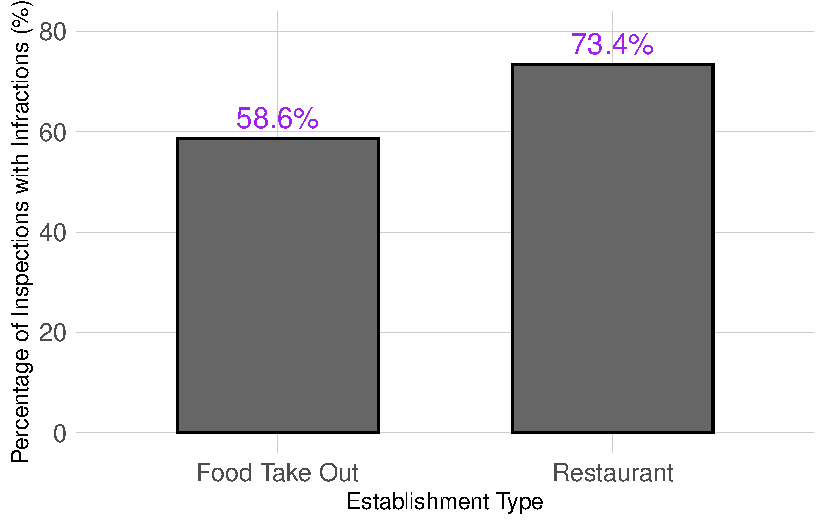
\includegraphics{paper_files/figure-pdf/fig-restaurant-vs-takeout-1.pdf}

}

\caption{\label{fig-restaurant-vs-takeout}Percentage of Inspections
Resulting in Infractions: Restaurants vs.~Takeout}

\end{figure}%

As shown in Figure~\ref{fig-restaurant-vs-takeout}, the percentage of
inspections resulting in infractions is higher for restaurants (73.4\%)
compared to takeout establishments (58.6\%). This indicates that despite
takeout establishments being subject to fewer total inspections due to
their smaller numbers, restaurants have a greater percentage of
infractions per inspection. This could suggest that full-service
restaurants face more complex operational challenges that increase the
likelihood of non-compliance with food safety regulations. Research has
shown that full-service restaurants, due to the complexity of food
handling processes, tend to have higher rates of infractions compared to
smaller or more specialized establishments (Analytics 2023; Agency
2023). These findings underscore the need for continued regulatory focus
on restaurants, where maintaining compliance appears more difficult,
reflecting the operational differences between full-service restaurants
and takeout locations (Centers for Disease Control and Prevention 2024).

\newpage

\section{Discussion}\label{sec-discussion}

The analysis of the DineSafe data revealed several key insights into
food safety practices across Toronto's restaurants and takeout
establishments. One notable observation, as depicted in
Figure~\ref{fig-inspection-vs-infraction} and discussed in
Section~\ref{sec-data-results}, is the positive correlation between the
number of inspections conducted at an establishment and the number of
infractions identified. This finding suggests that more frequent
inspections tend to uncover more infractions. However, it raises the
question of whether these inspections are uncovering ongoing compliance
issues rather than fostering improvements. Similar conclusions have been
noted in previous studies, which found that increased inspection
frequency highlights existing compliance problems without necessarily
reducing the overall number of violations (Public Health 2023; Centers
for Disease Control and Prevention 2024).

When examining the number of inspections conducted over time, as shown
in Figure~\ref{fig-inspections-over-time}, and detailed in
Section~\ref{sec-data-results}, the data indicates inconsistencies in
inspection activity. These variations are likely influenced by external
factors such as regulatory changes, public health events (e.g., the
COVID-19 pandemic), or operational adjustments (Analytics 2023). While
spikes in inspection activity may correspond to heightened public health
concerns, ensuring sustained compliance requires consistent follow-up
actions. Without continuous enforcement measures, temporary increases in
inspections may not lead to long-term reductions in infractions.

Figure~\ref{fig-restaurant-vs-takeout} in Section~\ref{sec-data-results}
compares the percentage of inspections resulting in infractions between
restaurants and takeout establishments. Restaurants, with a 73.4\%
infraction rate compared to 58.6\% for takeout establishments
(Figure~\ref{fig-restaurant-vs-takeout}), face greater compliance
challenges, suggesting a need for enhanced regulatory scrutiny. This
suggests that full-service restaurants, due to their operational
complexity, may face greater compliance challenges with food safety
regulations. This observation is consistent with other research that
highlights the difficulties full-service restaurants experience in
maintaining hygiene and safety standards, as their more complex
operations involve multiple stages of food preparation and handling
(Analytics 2023; Agency 2023). These findings underscore the importance
of focused regulatory oversight on restaurants, where compliance
challenges appear more prevalent.

Despite the valuable insights provided by this analysis, certain
limitations must be acknowledged. As noted in
Section~\ref{sec-data-results}, the DineSafe dataset may not capture all
infractions, especially for establishments classified as low-risk and
inspected less frequently. This underrepresentation could result in an
incomplete view of food safety compliance across the city. Moreover,
some infractions may not lead to immediate enforcement actions (e.g.,
fines or closures), potentially allowing non-compliance to persist over
time. Addressing these limitations may require additional measures such
as follow-up inspections and broadening the range of establishments
subject to frequent scrutiny (Gelfand 2022).

Future research could investigate the application of machine learning
techniques to predict which establishments are most likely to fail
inspections based on historical data, allowing regulatory bodies to
allocate resources more efficiently (Public Health 2023). Additionally,
more detailed studies into the effectiveness of enforcement actions,
such as fines and mandatory re-inspections, could provide insights into
strategies for improving compliance rates. Comparative analyses between
cities with varying levels of transparency, such as public disclosure of
inspection scores, could further illuminate best practices for reducing
foodborne illness outbreaks and enhancing compliance, as discussed in
Section~\ref{sec-discussion}.

In conclusion, while the DineSafe program has been successful in
identifying non-compliant establishments, this study suggests that
frequent inspections alone are not enough to prevent food safety
violations. Targeted regulatory interventions, particularly in high-risk
and complex food service sectors like full-service restaurants, may be
required to strengthen compliance and safeguard public health in
Toronto.

\newpage

\appendix

\section{Appendix}\label{sec-appendix}

\subsection{Dataset and Graph Sketches}\label{sec-appendix-sketches}

Sketches depicting both the desired dataset and the graphs generated in
this analysis are available in the GitHub Repository.

\subsection{Data Cleaning}\label{sec-appendix-cleaning}

The data cleaning process was essential to prepare the raw DineSafe
dataset for accurate analysis. Initially, we filtered the data to focus
exclusively on ``Restaurant'' and ``Food Take Out'' establishments that
had passed their most recent inspection. This ensured that our analysis
targeted establishments in good standing, allowing us to assess how
inspection frequency correlates with violations in compliant
establishments.

Next, we removed irrelevant columns to simplify the dataset and enhance
clarity. For example, columns unrelated to inspection outcomes or
establishment types were excluded. Additionally, we ensured consistency
across the dataset by renaming certain columns for clarity and ease of
analysis.

To handle date-related data, we utilized the lubridate package
(Grolemund and Wickham 2011), which enabled consistent date formatting
and facilitated time-based analysis. The entire data cleaning process
was carried out using the tidyverse package (Hadley Wickham et al.
2019), which streamlined the filtering, mutating, and summarizing
operations essential for preparing the dataset for further exploration.

\subsection{Attribution Statement}\label{sec-appendix-attribution}

``Contains information licensed under the Open Government Licence --
Toronto'' (Toronto 2024).

\newpage

\section*{References}\label{sec-references}
\addcontentsline{toc}{section}{References}

\phantomsection\label{refs}
\begin{CSLReferences}{1}{0}
\bibitem[\citeproctext]{ref-fsa2023}
Agency, Food Standards. 2023. {``The Impact of Displaying Food Hygiene
Ratings on Compliance.''} \emph{FSA Research and Evidence}.
\url{https://science.food.gov.uk/}.

\bibitem[\citeproctext]{ref-hazel2023}
Analytics, Hazel. 2023. {``Post-Pandemic Food Safety Compliance: Key
Insights from Health Inspections.''} \emph{Nation's Restaurant News}.
\url{https://www.nrn.com/food-safety/post-pandemic-food-safety-compliance}.

\bibitem[\citeproctext]{ref-cdc2024}
Centers for Disease Control and Prevention. 2024. {``Posting Inspection
Scores Reduces Foodborne Illness Outbreaks in Restaurants.''} \emph{Food
Safety Insights}. \url{https://www.cdc.gov/foodsafety/}.

\bibitem[\citeproctext]{ref-citeOpendatatoronto}
Gelfand, D. 2022. \emph{Opendatatoronto: Access the Toronto Open Data
Portal}. \url{https://CRAN.R-project.org/package=opendatatoronto}.

\bibitem[\citeproctext]{ref-citeLubridate}
Grolemund, Garrett, and Hadley Wickham. 2011. \emph{Lubridate: Make
Dealing with Dates a Little Easier}.
\url{https://CRAN.R-project.org/package=lubridate}.

\bibitem[\citeproctext]{ref-mdpi2023}
Public Health, MDPI Journal of. 2023. {``Using Machine Learning to
Predict Non-Compliant Food Outlets.''} \emph{MDPI Open Access}.
\url{https://www.mdpi.com/journal/publichealth}.

\bibitem[\citeproctext]{ref-citeR}
R Core Team. 2023. \emph{R: A Language and Environment for Statistical
Computing}. Vienna, Austria: R Foundation for Statistical Computing.
\url{https://www.R-project.org/}.

\bibitem[\citeproctext]{ref-tphlicense}
Toronto, City of. 2024. {``Open Government Licence -- Toronto.''}
\url{https://open.toronto.ca/open-data-license/}.

\bibitem[\citeproctext]{ref-citeGgplot2}
Wickham, H. 2016. \emph{Ggplot2: Elegant Graphics for Data Analysis}.
Springer-Verlag New York. \url{https://ggplot2.tidyverse.org}.

\bibitem[\citeproctext]{ref-citeTidyverse}
Wickham, Hadley, Mara Averick, Jennifer Bryan, Winston Chang, Lucy
D'Agostino McGowan, Romain François, Garrett Grolemund, et al. 2019.
{``Welcome to the {tidyverse}.''} \emph{Journal of Open Source Software}
4 (43): 1686. \url{https://doi.org/10.21105/joss.01686}.

\end{CSLReferences}




\end{document}
